\documentclass{standalone}
\usepackage{tikz}
\usetikzlibrary{patterns, positioning}


\begin{document}
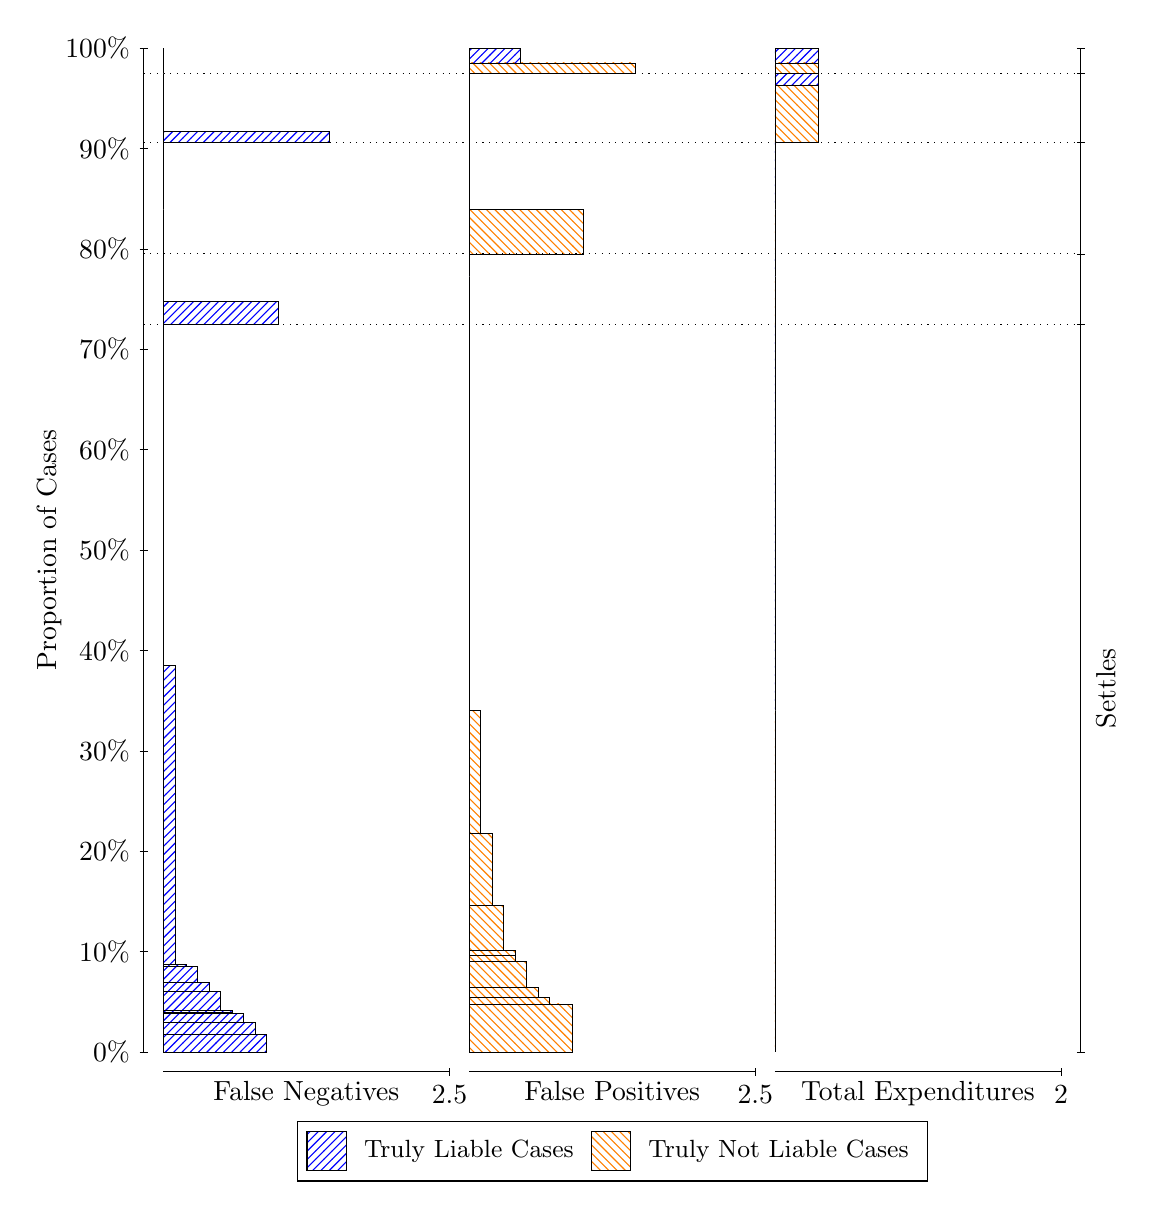
\begin{tikzpicture}
\draw[black, very thin] (1.5,1.75) -- (1.5,14.5);
\node[rotate=90, text=black, anchor=center] at (0.3, 8.125) {Proportion of Cases};
\draw[black, very thin] (1.45,1.75) -- (1.55,1.75);
\node[text=black, anchor=east] at (1.45, 1.75) {0\%};
\draw[black, very thin] (1.45,3.025) -- (1.55,3.025);
\node[text=black, anchor=east] at (1.45, 3.025) {10\%};
\draw[black, very thin] (1.45,4.3) -- (1.55,4.3);
\node[text=black, anchor=east] at (1.45, 4.3) {20\%};
\draw[black, very thin] (1.45,5.575) -- (1.55,5.575);
\node[text=black, anchor=east] at (1.45, 5.575) {30\%};
\draw[black, very thin] (1.45,6.85) -- (1.55,6.85);
\node[text=black, anchor=east] at (1.45, 6.85) {40\%};
\draw[black, very thin] (1.45,8.125) -- (1.55,8.125);
\node[text=black, anchor=east] at (1.45, 8.125) {50\%};
\draw[black, very thin] (1.45,9.4) -- (1.55,9.4);
\node[text=black, anchor=east] at (1.45, 9.4) {60\%};
\draw[black, very thin] (1.45,10.675) -- (1.55,10.675);
\node[text=black, anchor=east] at (1.45, 10.675) {70\%};
\draw[black, very thin] (1.45,11.95) -- (1.55,11.95);
\node[text=black, anchor=east] at (1.45, 11.95) {80\%};
\draw[black, very thin] (1.45,13.225) -- (1.55,13.225);
\node[text=black, anchor=east] at (1.45, 13.225) {90\%};
\draw[black, very thin] (1.45,14.5) -- (1.55,14.5);
\node[text=black, anchor=east] at (1.45, 14.5) {100\%};

\draw[black, very thin] (13.4,1.75) -- (13.4,14.5);
\draw[black, very thin] (13.35,1.75) -- (13.45,1.75);
\node[anchor=west] at (13.35, 1.75) {};
\draw[black, very thin] (13.35,10.991) -- (13.45,10.991);
\node[anchor=west] at (13.35, 10.991) {};
\draw[black, very thin] (13.35,11.885) -- (13.45,11.885);
\node[anchor=west] at (13.35, 11.885) {};
\draw[black, very thin] (13.35,13.302) -- (13.45,13.302);
\node[anchor=west] at (13.35, 13.302) {};
\draw[black, very thin] (13.35,14.174) -- (13.45,14.174);
\node[anchor=west] at (13.35, 14.174) {};
\draw[black, very thin] (13.35,14.5) -- (13.45,14.5);
\node[anchor=west] at (13.35, 14.5) {};

\draw[black, very thin, pattern color=blue, pattern=north east lines] (1.75,1.75) rectangle (3.058,1.9712);
\draw[black, very thin, pattern color=blue, pattern=north east lines] (1.75,1.9712) rectangle (2.9127,2.1211);
\draw[black, very thin, pattern color=blue, pattern=north east lines] (1.75,2.1211) rectangle (2.7673,2.2431);
\draw[black, very thin, pattern color=blue, pattern=north east lines] (1.75,2.2431) rectangle (2.622,2.2562);
\draw[black, very thin, pattern color=blue, pattern=north east lines] (1.75,2.2562) rectangle (2.622,2.2812);
\draw[black, very thin, pattern color=blue, pattern=north east lines] (1.75,2.2812) rectangle (2.4767,2.5229);
\draw[black, very thin, pattern color=blue, pattern=north east lines] (1.75,2.5229) rectangle (2.3313,2.6325);
\draw[black, very thin, pattern color=blue, pattern=north east lines] (1.75,2.6325) rectangle (2.186,2.8373);
\draw[black, very thin, pattern color=blue, pattern=north east lines] (1.75,2.8373) rectangle (2.0407,2.86);
\draw[black, very thin, pattern color=blue, pattern=north east lines] (1.75,2.86) rectangle (1.8953,6.6563);
\draw[black, very thin, pattern color=orange, pattern=north west lines] (1.75,6.6563) rectangle (1.75,10.991);
\draw[black, very thin, pattern color=blue, pattern=north east lines] (1.75,10.991) rectangle (3.2033,11.278);
\draw[black, very thin, pattern color=orange, pattern=north west lines] (1.75,11.278) rectangle (1.75,11.885);
\draw[black, very thin, pattern color=orange, pattern=north west lines] (1.75,11.885) rectangle (1.75,12.45);
\draw[black, very thin, pattern color=blue, pattern=north east lines] (1.75,12.45) rectangle (1.75,13.302);
\draw[black, very thin, pattern color=blue, pattern=north east lines] (1.75,13.302) rectangle (3.8573,13.443);
\draw[black, very thin, pattern color=orange, pattern=north west lines] (1.75,13.443) rectangle (1.75,14.174);
\draw[black, very thin, pattern color=orange, pattern=north west lines] (1.75,14.174) rectangle (1.75,14.311);
\draw[black, very thin, pattern color=blue, pattern=north east lines] (1.75,14.311) rectangle (1.75,14.5);
\draw[black, very thin, pattern color=orange, pattern=north west lines] (5.6333,1.75) rectangle (6.9413,2.3522);
\draw[black, very thin, pattern color=orange, pattern=north west lines] (5.6333,2.3522) rectangle (6.796,2.3612);
\draw[black, very thin, pattern color=orange, pattern=north west lines] (5.6333,2.3612) rectangle (6.6507,2.4433);
\draw[black, very thin, pattern color=orange, pattern=north west lines] (5.6333,2.4433) rectangle (6.5053,2.5714);
\draw[black, very thin, pattern color=orange, pattern=north west lines] (5.6333,2.5714) rectangle (6.36,2.8959);
\draw[black, very thin, pattern color=orange, pattern=north west lines] (5.6333,2.8959) rectangle (6.2147,2.9739);
\draw[black, very thin, pattern color=orange, pattern=north west lines] (5.6333,2.9739) rectangle (6.2147,3.0391);
\draw[black, very thin, pattern color=orange, pattern=north west lines] (5.6333,3.0391) rectangle (6.0693,3.6144);
\draw[black, very thin, pattern color=orange, pattern=north west lines] (5.6333,3.6144) rectangle (5.924,4.5277);
\draw[black, very thin, pattern color=orange, pattern=north west lines] (5.6333,4.5277) rectangle (5.7787,6.0851);
\draw[black, very thin, pattern color=blue, pattern=north east lines] (5.6333,6.0851) rectangle (5.6333,10.991);
\draw[black, very thin, pattern color=orange, pattern=north west lines] (5.6333,10.991) rectangle (5.6333,11.598);
\draw[black, very thin, pattern color=blue, pattern=north east lines] (5.6333,11.598) rectangle (5.6333,11.885);
\draw[black, very thin, pattern color=orange, pattern=north west lines] (5.6333,11.885) rectangle (7.0867,12.45);
\draw[black, very thin, pattern color=blue, pattern=north east lines] (5.6333,12.45) rectangle (5.6333,13.302);
\draw[black, very thin, pattern color=orange, pattern=north west lines] (5.6333,13.302) rectangle (5.6333,14.033);
\draw[black, very thin, pattern color=blue, pattern=north east lines] (5.6333,14.033) rectangle (5.6333,14.174);
\draw[black, very thin, pattern color=orange, pattern=north west lines] (5.6333,14.174) rectangle (7.7407,14.311);
\draw[black, very thin, pattern color=blue, pattern=north east lines] (5.6333,14.311) rectangle (6.2873,14.5);
\draw[black, very thin, pattern color=orange, pattern=north west lines] (9.5167,1.75) rectangle (9.5167,6.0851);
\draw[black, very thin, pattern color=blue, pattern=north east lines] (9.5167,6.0851) rectangle (9.5167,10.991);
\draw[black, very thin, pattern color=orange, pattern=north west lines] (9.5167,10.991) rectangle (9.5167,11.598);
\draw[black, very thin, pattern color=blue, pattern=north east lines] (9.5167,11.598) rectangle (9.5167,11.885);
\draw[black, very thin, pattern color=orange, pattern=north west lines] (9.5167,11.885) rectangle (9.5167,12.45);
\draw[black, very thin, pattern color=blue, pattern=north east lines] (9.5167,12.45) rectangle (9.5167,13.302);
\draw[black, very thin, pattern color=orange, pattern=north west lines] (9.5167,13.302) rectangle (10.062,14.033);
\draw[black, very thin, pattern color=blue, pattern=north east lines] (9.5167,14.033) rectangle (10.062,14.174);
\draw[black, very thin, pattern color=orange, pattern=north west lines] (9.5167,14.174) rectangle (10.062,14.311);
\draw[black, very thin, pattern color=blue, pattern=north east lines] (9.5167,14.311) rectangle (10.062,14.5);
\draw[black, dotted] (1.5,10.991) -- (13.4,10.991);
\draw[black, dotted] (1.5,11.885) -- (13.4,11.885);
\draw[black, dotted] (1.5,13.302) -- (13.4,13.302);
\draw[black, dotted] (1.5,14.174) -- (13.4,14.174);
\draw[black, very thin] (1.75,1.5) -- (5.3833,1.5);
\node[text=black, anchor=north] at (3.5667, 1.5) {False Negatives};
\draw[black, very thin] (5.3833,1.45) -- (5.3833,1.55);
\node[text=black, anchor=north] at (5.3833, 1.45) {2.5};

\draw[black, very thin] (5.6333,1.5) -- (9.2667,1.5);
\node[text=black, anchor=north] at (7.45, 1.5) {False Positives};
\draw[black, very thin] (9.2667,1.45) -- (9.2667,1.55);
\node[text=black, anchor=north] at (9.2667, 1.45) {2.5};

\draw[black, very thin] (9.5167,1.5) -- (13.15,1.5);
\node[text=black, anchor=north] at (11.333, 1.5) {Total Expenditures};
\draw[black, very thin] (13.15,1.45) -- (13.15,1.55);
\node[text=black, anchor=north] at (13.15, 1.45) {2};

\node[text=black, centered, rotate=90] at (13.72, 6.3707) {Settles};





\draw (7.449999999999999,1.5) node[draw=none] (baseCoordinate) {};
\begin{scope}[align=center]
        \matrix[scale=0.5, draw=black, below=0.5cm of baseCoordinate, nodes={draw}, column sep=0.1cm]{
            \node[rectangle, draw, minimum width=0.5cm, minimum height=0.5cm, pattern color=blue, pattern=north east lines] {}; &
            \node[draw=none, font=\small, text=black] (B) {Truly Liable Cases}; &
            \node[rectangle, draw, minimum width=0.5cm, minimum height=0.5cm, pattern color=orange, pattern=north west lines] {}; &
            \node[draw=none, font=\small, text=black] (B) {Truly Not Liable Cases}; \\
            };
\end{scope}

\end{tikzpicture}
\end{document}